\newpage
\section{Общие сведения о системе}
\subsection{Авторизация пользователей}
\subsubsection{Вход в систему} \label{p_gen_entry}

Перед началом работы в \tmis ~необходимо зарегистрироваться у администратора системы. Во время регистрации пользователю будет присвоен персональный идентификатор и пароль.

\begin{vnim}
 Персональный идентификатор и пароль предназначены для индивидуального доступа в систему. Никогда не сообщайте их третьим лицам!
\end{vnim}

\begin{figure}[ht]\centering
 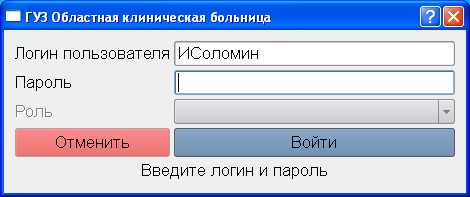
\includegraphics[width = 0.8\textwidth ,keepaspectratio]{p_gen_entry}
 \caption{Окно авторизации пользователя в \tmis}
 \label{img_gen_entry}
\end{figure} 
    
Для начала сеанса работы с \tmis , требуется выполнить вход в систему. Процедура входа в систему называется авторизацией и состоит из следующих шагов:
\begin{enumerate}
\item Запустить приложение \tmis, используя соответствующий ярлык на рабочем столе.
\item В открывшемся окне (Рисунок \ref{img_gen_entry}) нужно ввести идентификатор пользователя, пароль и нажать кнопку \btn{Войти}.
\item Если пользователь в системе выполняет только одну роль, то окно авторизации исчезнет и пользователю станет доступно главное окно программы (Рисунок \ref{img_gen_mw}). В случае если у пользователя имеется несколько ролей, требуется выбрать роль из выпадающего списка (Рисунок \ref{img_gen_entry_rol}) и нажать кнопку  \btn{Выбрать}, после чего пользователю так же станет доступно главное окно программы (Рисунок \ref{img_gen_mw}).
\end{enumerate}
 
\begin{figure}[ht]\centering
 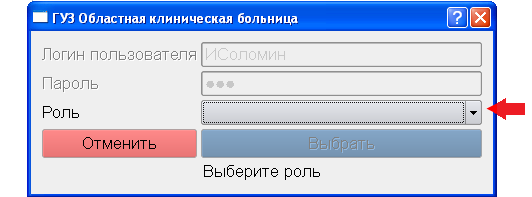
\includegraphics[width = 0.9\textwidth ,keepaspectratio]{p_gen_entry_rol}
 \caption{Выбор роли пользователя}
 \label{img_gen_entry_rol}
\end{figure} 

\begin{figure}[ht]\centering
 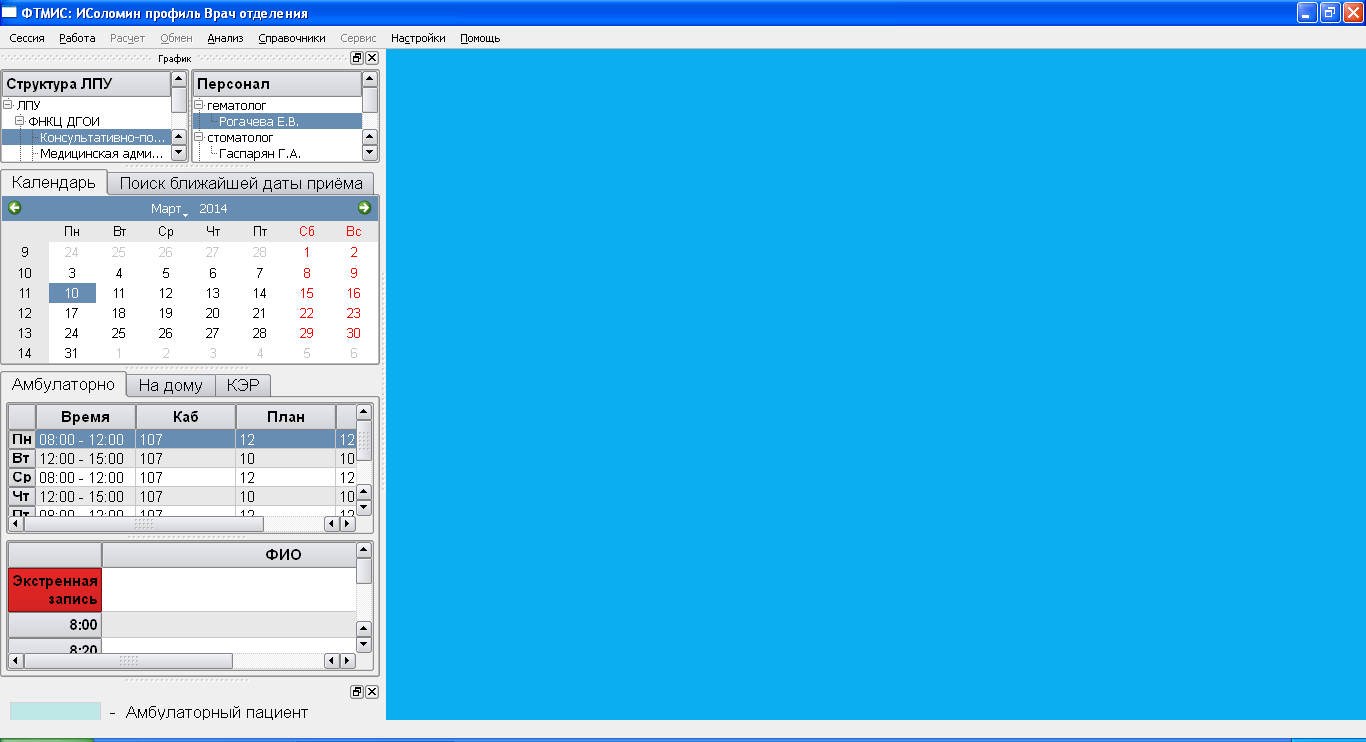
\includegraphics[width = 1\textwidth ,keepaspectratio]{p_gen_mw}
 \caption{Главное окно программы}
 \label{img_gen_mw}
\end{figure} 

Если были введены неверные идентификатор пользователя и (или) пароль, на экране появится сообщение об ошибке (Рисунок \ref{img_gen_entry_err}).

\begin{figure}[ht]\centering
 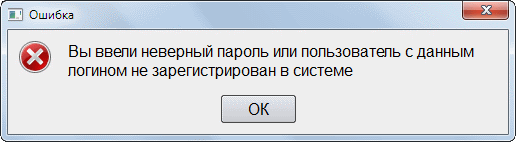
\includegraphics[width = 0.6\textwidth ,keepaspectratio]{p_gen_entry_err}
 \caption{Сообщение об ошибке авторизации}
 \label{img_gen_entry_err}
\end{figure} 

При возникновении данной ошибки рекомендуется:
\begin{itemize}
 \item Проверить язык ввода.
 \item Проверить состояние клавиши \keys{CapsLock} на клавиатуре и выключить ее при необходимости. 
 \item Если в пароле присутствуют цифры, проверить состояние клавиши \keys{NumLock}, включить ее при необходимости.
 \item Повторить попытку авторизации.
\end{itemize}
 
Если проблема не была решена, нужно обратиться к администратору системы для проверки идентификационных данных.

Если в окне авторизации пользователя была нажата кнопка \btn{Отменить} , то основное окно программы останется открытым, но все функции работы в системе будут недоступны. Повторный вход в систему описан в разделе \ref{p_gen_reentry}

\subsubsection{Завершение работы}

\begin{vnim}
Перед закрытием приложения рекомендуется  сохранить все сделанные изменения и закрыть все активные окна.
\end{vnim}

Для выхода из программы необходимо выбрать в главном меню пункт \mm{Сессия \str Закрыть программу} либо нажать кнопку \btn{x}   в правом верхнем углу главного окна. В результате описанных действий программа будет закрыта без дополнительных предупреждений.

\subsubsection{Смена имени пользователя} \label{p_gen_reentry}

Вход в систему под другим именем пользователя можно выполнить не прибегая к закрытию приложения, используя функцию отключения и повторного подключения к базе данных.

Для выхода из системы текущего пользователя нужно в главном меню выбрать \mm{Сессия \str Отключиться от базы данных}. При этом станет недоступной информация на панели слева и большинство пунктов главного меню.

Для входа в систему под новым именем пользователя требуется в главном меню выбрать \mm{Сессия \str Подключиться к базе данных}. На экране появится окно авторизации, куда нужно ввести идентификатор и пароль нового пользователя. Подробно процедура авторизации рассмотрена в разделе \ref{p_gen_entry} Так же рекомендуется использовать команду подключения к базе данных, если во время авторизации пользователя была нажата кнопка \btn{Отменить}.
